%\documentclass[envcountsect,handout]{beamer}
\documentclass[envcountsect]{beamer}
%\setbeamertemplate{theorems}[numbered]
\usetheme{Boadilla} %{Madrid}
% Tikz graphics - should these be imported as images instead?
\usepackage{graphicx, tikz}
\usetikzlibrary{shapes, arrows, positioning, calc}
% Citations
\usepackage[style = authoryear]{biblatex}
\addbibresource{bibliography.bib}

\usepackage{mathtools}
\DeclareMathOperator*{\argmax}{arg\,max}

\title{Introduction to Part-of-Speech Tagging}
\subtitle{Graphical Models and Algorithms for Sequence Labelling}
\author{Alex Simcock}
\institute{University of Birmingham}
\date{\today}

\begin{document}

\begin{frame}
\titlepage
\end{frame}

\begin{frame}{Part-of-Speech Tagging}

\begin{definition}[Part-of-Speech]
The term `part-of-speech' refers to the syntactic category of a word, for example noun, verb or adjective.
\end{definition}

\begin{example}[Ambiguous Parts-of-Speech]
\begin{center}
\begin{tabular}{ c c c c c }
 `The & fans & watch & the & race' \\
 \hline
 \textbf{Dt} & \textbf{Nn} & \textbf{Nn} & \textbf{Dt} & \textbf{Nn} \\  
 & \textbf{Vb} & \textbf{Vb} & & \textbf{Vb}    
\end{tabular}
\end{center}
\end{example}

How can we best label any given word sequence in the presence of grammatical-ambiguity?

%Part-of-speech tagging is a key preliminary step in many natural language processing pipelines.

\end{frame}

\begin{frame}

\begin{definition}[POS Tagging as Structure Prediction]

Let $X$ and $Y$ be random variables such that $X$ varies over all word sequences and $Y$ over all label sequences.
\begin{align*}
    X &= (x_k)_{k=1}^n = (\text{`the'}, \text{`fans'}, \text{`watch'}, \text{`the'}, \text{`race'}) \\
    Y &= (y_k)_{k=1}^n = (\textbf{Dt}, \textbf{Nn}, \textbf{Nn}, \textbf{Dt}, \textbf{Nn}), \quad y_k \in \mathcal{Y}
\end{align*}

The POS tagging problem can now be written:

`\textbf{Given $X$, predict the correctly matched tag sequence $Y$}'.

\end{definition}

\pause

\textbf{Maximum likelihood estimation} tells us that the best choice of $Y$ will maximise the probability of observing our word sequence:
\begin{equation*}
    Y^* \coloneqq \argmax_{Y} p(Y \mid X)
\end{equation*}    

\end{frame}

\begin{frame}{The Na{\"i}ve Bayes Classifier}

\begin{definition}[Na{\"i}ve Bayes Classifier]
    Na{\"i}ve Bayes models the joint probability distribution $p(X,Y)$:
    \begin{equation*}
        p(X,Y) = \prod_{i=1}^n p(X_i \mid Y_i)p(Y_i)
    \end{equation*}
\end{definition}

\pause

We can apply the Na{\"i}ve Bayes model to derive $Y^*$,
\begin{gather*}
    p(Y \mid X) = \frac{p(Y,X)}{p(X)} = \frac{1}{p(X)}\prod_{i=1}^n p(X_i \mid Y_i)p(Y_i) = \frac{1}{p(X)}\prod_{i=1}^n p(X_i, Y_i) \\
    \therefore Y^* = \argmax_Y p(Y \mid X) = \argmax_Y \prod_{i=1}^n p(X_i, Y_i)
\end{gather*}

\pause

The result is a model which simply selects the most common tag for each word!

\end{frame}

\begin{frame}{Na{\"i}ve Bayes as a Graphical Model}

\begin{figure}[ht]
\centering
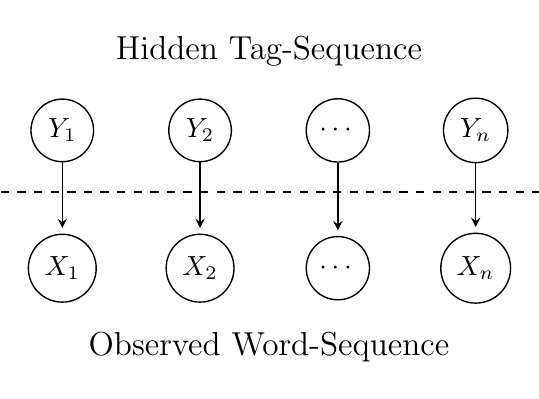
\begin{tikzpicture} [-> , >= stealth, shorten >= 2 pt, line width = 0.5pt, node distance = 1.75cm]

\node [draw, circle] (y1) {$Y_1$};
\node [draw, circle] (y2) [right of = y1] {$Y_2$};
\node [draw, circle] (ydot) [right of = y2] {$\cdots$};
\node [draw, circle] (yn) [right of = ydot] {$Y_n$};

\node [draw, circle] (x1) [below of = y1] {$X_1$};
\node [draw, circle] (x2) [below of = y2] {$X_2$};
\node [draw, circle] (xdot) [below of = ydot] {$\cdots$};
\node [draw, circle] (xn) [below of = yn] {$X_n$};

\path (y1) edge (x1);
\path (y2) edge (x2);
\path (ydot) edge (xdot);
\path (yn) edge (xn);


\node (c1w1) at ($(y1)!0.45!(x1)$) {};
\node (c3w3) at ($(yn)!0.45!(xn)$) {};
\draw [-, dashed, line width =0.75 pt, shorten >=-1.75cm, shorten <=-1.75cm] (c1w1) -- (c3w3);

\node (y2.5) at ($(y2)!0.5!(ydot)$) {};
\node (x2.5) at ($(x2)!0.5!(xdot)$) {};
\node [above of = y2.5, node distance= 1cm] {\large Hidden Tag-Sequence};
\node [below of = x2.5, node distance= 1cm] {\large Observed Word-Sequence};

\end{tikzpicture}
\end{figure}

\end{frame}

\begin{frame}{The Hidden Markov Model (HMM)}

\begin{figure}[ht]
\centering
\hspace{-1.9cm}
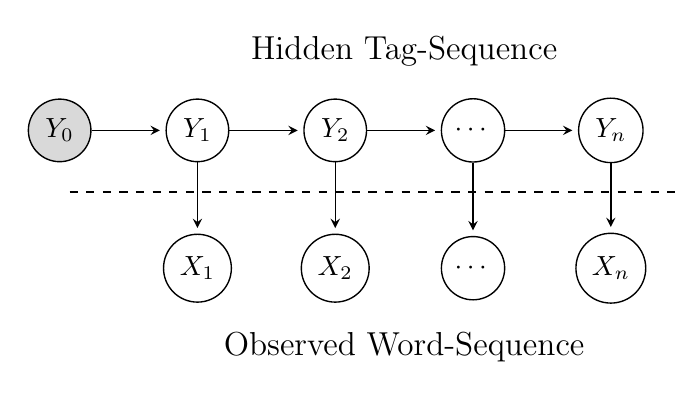
\begin{tikzpicture} [-> , >= stealth, shorten >= 2 pt, line width = 0.5pt, node distance = 1.75cm]

\node [draw, circle] (y1) {$Y_1$};
\node (start) [draw, circle, fill=gray!30!white, left of = y1] {$Y_0$};
\node [draw, circle] (y2) [right of = y1] {$Y_2$};
\node [draw, circle] (ydot) [right of = y2] {$\cdots$};
\node [draw, circle] (yn) [right of = ydot] {$Y_n$};

\path (start) edge (y1);
\path (y1) edge (y2);
\path (y2) edge (ydot);
\path (ydot) edge (yn);

\node [draw, circle] (x1) [below of = y1] {$X_1$};
\node [draw, circle] (x2) [below of = y2] {$X_2$};
\node [draw, circle] (xdot) [below of = ydot] {$\cdots$};
\node [draw, circle] (xn) [below of = yn] {$X_n$};

\path (y1) edge (x1);
\path (y2) edge (x2);
\path (ydot) edge (xdot);
\path (yn) edge (xn);


\node (c1w1) at ($(y1)!0.45!(x1)$) {};
\node (c3w3) at ($(yn)!0.45!(xn)$) {};
\draw [-, dashed, line width =0.75 pt, shorten >=-1.75cm, shorten <=-1.75cm] (c1w1) -- (c3w3);

\node (y2.5) at ($(y2)!0.5!(ydot)$) {};
\node (x2.5) at ($(x2)!0.5!(xdot)$) {};

\node [above of = y2.5, node distance= 1cm] {\large Hidden Tag-Sequence};
\node [below of = x2.5, node distance= 1cm] {\large Observed Word-Sequence};

\end{tikzpicture}
\end{figure}

\end{frame}

\begin{frame}

The HMM can be summarised by its key parameters, the sets of emission and transition probabilities: $A$ and $B$.

\begin{align*}
    A &= [ A_k(w) ] \quad k \in \mathcal{Y}, & \quad & A_k(w) = p(X_t = w \mid Y_t = k), \\
    B  &= [ B_{k,k'} ] \quad k, k' \in \mathcal{Y}, & \quad  & B_{k,k'} = p(Y_t = k' \mid Y_{t-1} = k), \\
    \pi &= [ \pi_k ] \quad k \in \mathcal{Y}, & \quad & \pi_k = p(Y_1 = k).
\end{align*}

\pause

There are three key questions for HMMs:
\begin{enumerate}
    \item Given the observed sequence $X$ and a HMM $\theta = (A, B, \pi)$, how do we efficiently compute $p(X \mid \theta)$?
    \item Given the observed sequence $X$ and a HMM $\theta$, how do we choose the corresponding state sequence $Y$ that best explains the observations?
    \item How might we adjust the model parameters in order to maximise $p(X \mid \theta)$?
\end{enumerate}

\end{frame}

\begin{frame}{The Forward-Backward Algorithm}

$p(X \mid \theta)$ is also the sum of $p(X, Y \mid \theta)$ over all possible state-sequences.

To derive this value we require two identities that result from the model assumptions of emission independence and markov property:
\begin{align*}
    p(X \mid Y, \theta) &= \prod_{i=1}^n p(X_i \mid Y_i, \theta) = \prod_{i=1}^n A_{Y_i}(X_i) \\
    p(Y \mid \theta) &= \pi_{Y_1} B_{Y_1,Y_2} \cdots B_{Y_{n-1},Y_n}
\end{align*}
These identities can then be applied as follows,
\begin{align*}
    p(X \mid \theta) &= \sum_{\forall \: Y} p(X,Y \mid \theta) = \sum_{\forall \: Y} p(X \mid Y, \theta) p(Y \mid \theta) \\
    &= \sum_{\forall \: Y} \pi_{Y_1} A_{Y_1}(X_1) B_{Y_1, Y_2} A_{Y_2}(X_2) \cdots B_{Y_{n-1}, Y_n} A_{Y_n}(X_n)
\end{align*}

\pause

This calculation is \textcolor{red}{intractable} and has exponential complexity $O(2n|\mathcal{Y}|^n)$.
% owing to the $2n - 1$ multiplications for each of the $|\mathcal{Y}|^n$ possible values of $Y$.

\end{frame}

\begin{frame}
    In order to calculate more efficiently we can apply dynamic programming:
    \begin{definition}[Forward-Function]
        Let $\alpha_t(k)$ denote the joint probability of observing the sequence $X_1 X_2 \cdots X_t \, (1 \leq t \leq n$) and the tag $Y_t$ being $k$, given model parameters $\theta$.
        \begin{equation*}
            \alpha_t(k) \coloneqq p(X_1,X_2,\ldots,X_t,Y_t=k \mid \theta)
        \end{equation*}
    \end{definition}

\pause

Having defined $\alpha_t(k)$, we note that $p(X \mid \theta) = \sum_{k \in \mathcal{Y}} \alpha_n(k)$, if we can efficiently solve for a given $\alpha_t(k)$ then we have answered the first question!

\pause

\begin{definition}[Forward-Algorithm]
Any value of $\alpha_t(k)$ can be found inductively:
\begin{align*}
    \alpha_1(k) &= \pi_{k} A_k(X_1) & \quad & \:\: k \in \mathcal{Y} \\
    \alpha_{t+1}(k) &= \left[ \sum_{k' \in \mathcal{Y}} \alpha_{t}(k')B_{k',k} \right] A_k(X_{t+1}) & \quad &
        \begin{array}{lr}
            1 \leq t \leq n-1\\
            k, k' \in \mathcal{Y}
        \end{array}
\end{align*}
\end{definition}

\end{frame}

\begin{frame}

This approach calculates $p(X \mid \theta)$ with complexity $O(n|\mathcal{Y}|^2)$.

Given a pre-trained HMM and the generic tagset of the British National Corpus we could now calculate the likelihood of generating `the fans watch the race' ($|\mathcal{Y}|=61,n=5$) with $10^{15}$ times less calculations!

\pause

\vspace{0.5cm}

$\alpha_t(k)$ is only the first of several helper variables that apply the principle of dynamic programming to speed up calculations for HMMs and other, more advanced graphical methods such as the Conditional Random Field (CRF).

\vspace{0.5cm}

The algorithms for tagging and training both HMMs and CRFs are discussed in full detail in my project and I recommend the papers \textit{`A tutorial on hidden Markov models and selected applications in speech recognition'} \footcite{rabiner-1989-tutorial} and \textit{`An introduction to conditional random fields'} \footcite{sutton-2012-crfintro} for comprehensive tutorials of the mathematics behind these models.

%At each step of induction we calculate the value $\alpha_t$ for all $|\mathcal{Y}|$ states, where each is derived from $|\mathcal{Y}|$ previous states.
%Carrying out this calculation for each of the $n-1$ steps results in overall complexity of order $O(n|\mathcal{Y}|^2)$.

\end{frame}

\begin{frame}
\begin{center}
    \huge Thank you for listening.
\end{center}
\end{frame}

\end{document}